\section{Extended Equations and Unit Notes}

The implementation uses SI units internally at solver boundaries. Voltages are converted from mV to V, capacitances from pF to F, conductances from nS to S, currents from pA to A, and time from ms to s. Geometry-derived neck resistance uses centimeters for $\rho_i$ compatibility:
\begin{equation}
\Rneck=\frac{\rho_i L_n}{\pi r_n^2}.
\end{equation}
For nonuniform neck profiles the code evaluates
\begin{equation}
\Rneck=\int_0^{L_n}\frac{\rho_i}{\pi r(x)^2}\,dx
\end{equation}
by numerical quadrature. Tapered, constricted, and profile-based necks preserve the intended geometry and report an effective resistance for comparison with lumped approximations.

The spine-omitted dendrite-soma load is a two-node DC circuit in the baseline reference case. With dendrite leak $g_{L,d}$, soma leak $g_{L,s}$, and dendrite-soma coupling $g_{ds}$, direct linear solution gives the dendritic one-port input resistance used in the main text:
\begin{equation}
\Rin =
\left(g_{L,d}+\frac{g_{ds}g_{L,s}}{g_{ds}+g_{L,s}}\right)^{-1}.
\end{equation}
Using the baseline values gives $\Rin=144.486692$ M$\Omega$, matching the Phase 4 direct DC solve to roundoff.

The analytic local divider is therefore
\begin{equation}
\Gamma_{\mathrm{div}}=\frac{\Rin}{\Rneck+\Rin}=\frac{1}{1+\SMI},
\end{equation}
and the manuscript residual is
\begin{equation}
\Delta_{\mathrm{div}}=\Ghd-\Gamma_{\mathrm{div}}.
\end{equation}
These equations define a DC small-signal reference. They do not assert that transient conductance-based peak transfer must equal the divider value.

The passive matrix in the main manuscript generalizes to an arbitrary passive tree as
\begin{equation}
\mathbf{C}\frac{d\mathbf{V}}{dt}=-\left(\mathbf{G}_L+\mathbf{G}_A+\mathbf{G}_{\mathrm{syn}}(t)\right)\mathbf{V}+\mathbf{b}(t),
\end{equation}
where $\mathbf{G}_A$ is assembled from axial edges. Each edge with conductance $g_{ij}$ contributes $+g_{ij}$ to both diagonal entries and $-g_{ij}$ to the symmetric off-diagonal entries. This construction preserves reciprocity in passive linear systems.

\begin{figure}[!htbp]
\centering
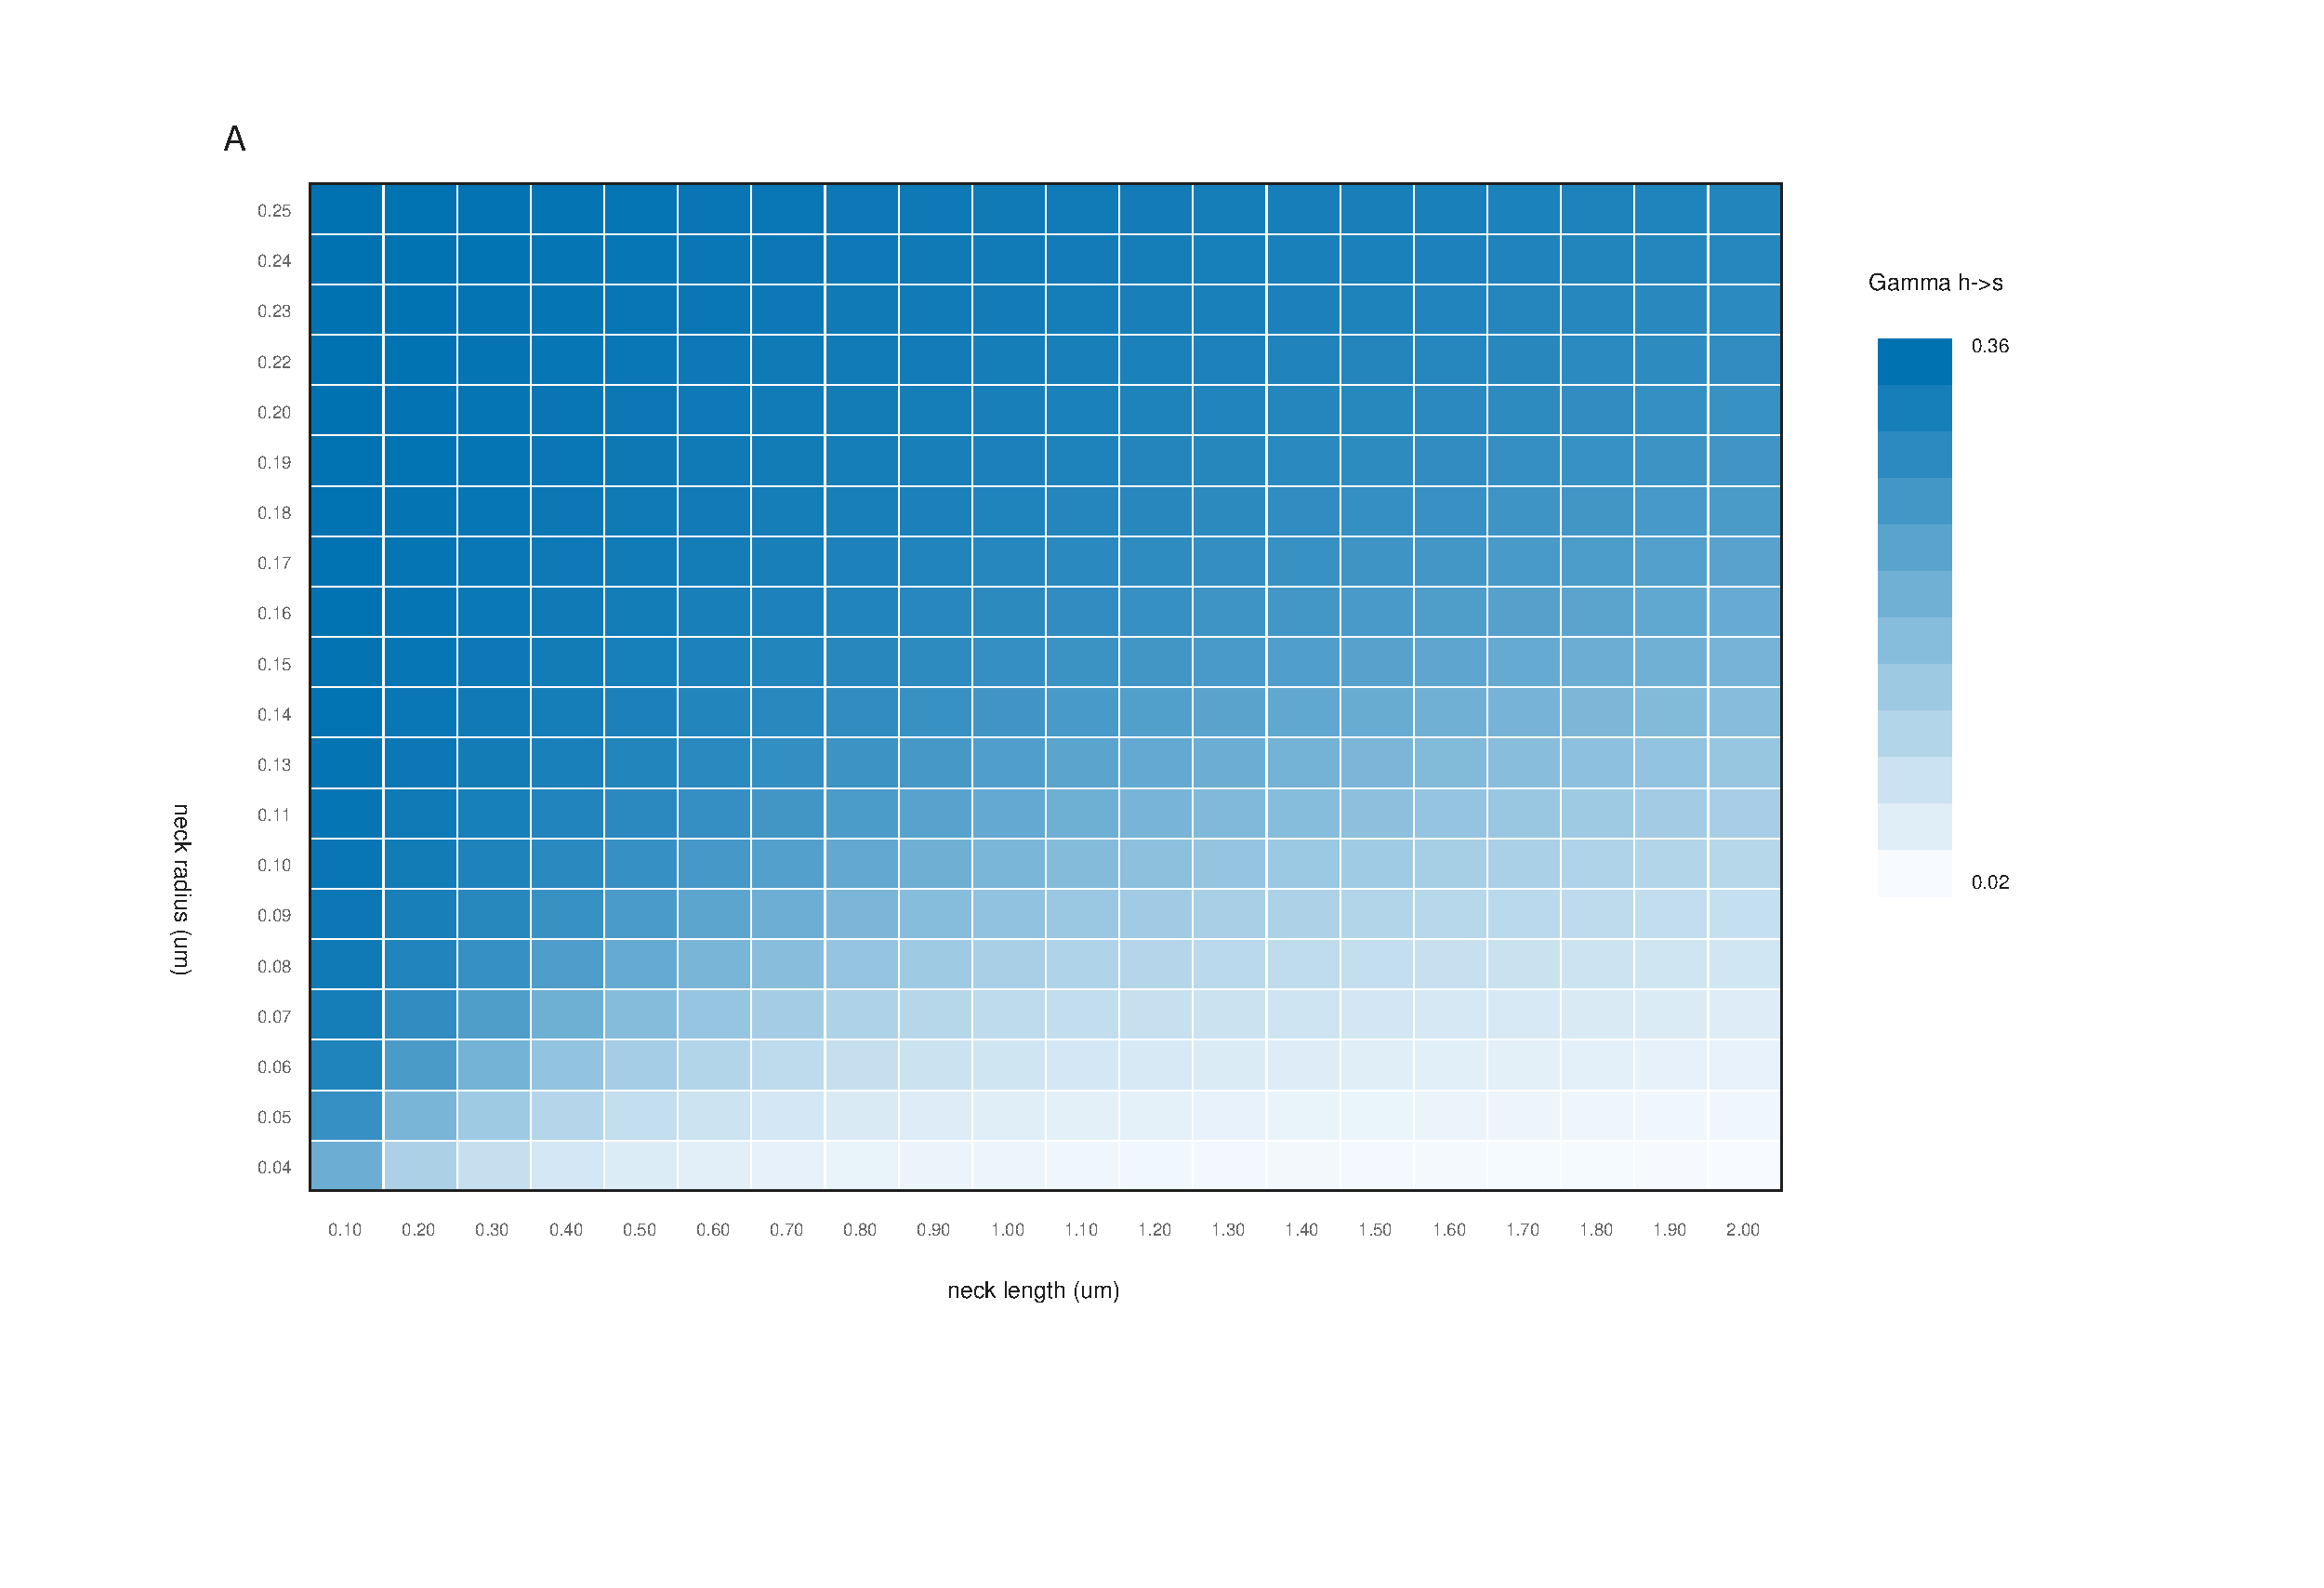
\includegraphics[width=0.9\textwidth,keepaspectratio]{../figures_publication/FigS1_fixed_load_heatmap.pdf}
\caption{\textbf{Figure S1.} Fixed-load head-to-soma transfer heatmap from the baseline validation sweep. The heatmap complements the main-text load-normalization controls by showing the two-parameter neck-geometry grid.}
\label{fig:s1_fixedload}
\end{figure}
